\documentclass[Ligatures=TeX,table,brazil,svgnames,usetotalslideindicator,compress,10pt]{beamer}

\usetheme[titleformat=allsmallcaps]{metropolis}

\usepackage{polyglossia}
\setdefaultlanguage{brazil}
\disablehyphenation

\usepackage{minted}

\usetikzlibrary{arrows,positioning,calc}

\usepackage{graphicx}
\graphicspath{{./figuras/}}
\usepackage{subcaption}
\usepackage{xmpmulti}

% \usepackage{textpos}

% \usepackage{mdwlist}
% \usepackage{siunitx}
\usepackage{alltt}
% \usepackage{multicol}
\usepackage{xspace}
\usepackage{multirow}
\usepackage{amsmath}

\usepackage{cancel}

\newcommand{\setcoverbg}{
  \setbeamertemplate{background}
  {\includegraphics[width=\paperwidth,height=\paperheight]{backgrounds/coverbg}}
}
\newcommand{\setintersectionbg}{
  \setbeamertemplate{background}
  {\includegraphics[width=\paperwidth,height=\paperheight]{backgrounds/blank}}
}
\newcommand{\setsectionbg}{
  \setbeamertemplate{background}
  {\includegraphics[width=\paperwidth,height=\paperheight]{backgrounds/slidebg2}}
}

\setbeamertemplate{caption}{default}

\title{MCTA025-13 - Sistemas Distribuídos}
\subtitle{Processos, Virtualização e Migração}

\author{Emilio Francesquini}
\institute{Centro de Matemática, Computação e Cognição\\ Universidade Federal do ABC}
\date{25 de junho de 2018}

\begin{document}

\setcoverbg
\maketitle

\setsectionbg

\begin{frame}
  \frametitle{Disclaimer}
  \begin{itemize}
  \item Estes slides foram preparados para o curso de \textbf{Sistemas
      Distribuídos na UFABC}.
  \item Este material pode ser usado livremente desde que sejam
    mantidos, além deste aviso, os créditos aos autores e
    instituições.
  \item Estes slides foram adaptados daqueles originalmente preparados
    (e gentilmente cedidos) pelo professor \textbf{Daniel Cordeiro, da
      EACH-USP} que por sua vez foram baseados naqueles
    disponibilizados online pelos autores do livro ``Distributed
    Systems'', 3ª Edição em:
    \url{https://www.distributed-systems.net}.
  \end{itemize}
\end{frame}



\begin{frame}
  \frametitle{Computadores de memória compartilhada}

  \begin{columns}
    \begin{column}{0.5\textwidth}
      \begin{itemize}
      \item Todas as posições de memória podem ser acessadas por todos as
        unidades de processamento
        \begin{itemize}
        \item \alert{Espaço de endereçamento único}
        \end{itemize}
      \item Symmetric Multiprocessing Platforms (SMP) são arquiteturas de
        memória compartilhada que possuem ao menos duas unidades de
        processamento
      \item \alert{UMA - Uniform Memory Access}
      \end{itemize}
    \end{column}
    \begin{column}{0.5\textwidth}
      \begin{figure}
        \centering
        \includegraphics[width=\textwidth]{uma}
      \end{figure}
     \end{column}
  \end{columns}
\end{frame}


\begin{frame}
  \frametitle{Arquiteturas NUMA}

  \begin{columns}
    \begin{column}{0.5\textwidth}
      \begin{itemize}
      \item \alert{NUMA – Non-Uniform Memory Access}
      \item Pode-se imaginar uma máquina NUMA como sendo um conjunto de máquinas UMA ligadas por uma rede de interconexão de alto desempenho
      \item \alert{Espaço de endereçamento único}
        \begin{itemize}
        \item \alert{Desempenho} para acesso à memória \alert{variável}
        \end{itemize}

      \end{itemize}
    \end{column}
    \begin{column}{0.5\textwidth}
      \begin{figure}
        \centering
        \includegraphics[width=\textwidth]{numa}
      \end{figure}
     \end{column}
  \end{columns}
\end{frame}

\begin{frame}
  \frametitle{Topologias NUMA}

  \begin{columns}
    \begin{column}{0.5\textwidth}
      \begin{itemize}
      \item Topologias comuns
        \begin{itemize}
        \item \alert{Toroidal}: Kalray MPPA-256
        \item \alert{Grade}: Tilera TILE-GX*
        \item \alert{Anel}: Intel Xeon Phi
        \item \alert{Hipercubo}: SGI Altix UV2000
        \end{itemize}
      \item \alert{Conhecimento da topologia é essencial} para desenvolver programas com um \alert{bom desempenho}
      \end{itemize}
    \end{column}
    \begin{column}{0.5\textwidth}
      \begin{figure}
        \centering
        \includegraphics[width=0.85\textwidth]{topo} \\
        \footnotesize{SGI Altix UV2000 – Hipercubo (5D) com conexões privilegiadas}
      \end{figure}
     \end{column}
  \end{columns}
\end{frame}


\begin{frame}
  \frametitle{Introdução a Processos e Threads}

  \begin{block}{Ideia básica}
    Construir um \alert{processador virtual} com software, em cima dos processadores físicos:
  \end{block}

  \begin{description}
  \item[processador:] (hardware) provê um conjunto de instruções junto
    com a capacidade de executá-las automaticamente
  \item[thread:] (software) um processador mínimo com um
    \alert{contexto} que possui uma série de instruções que podem ser
    executados. Gravar o contexto de um thread implica parar
    a execução e guardar todos os dados necessários para continuar a
    execução posteriormente
  \item[processo:] (software) um processador em cujo contexto pode ser
    executado uma ou mais threads. Executar um thread significa
    executar uma série de instruções no contexto daquele
    processo.
  \end{description}

\end{frame}

\begin{frame}
  \frametitle{Processos}
  \begin{itemize}
  \item Uma das abstrações mais importantes de um SO
    \begin{itemize}
    \item Representam \alert{a execução} de um programa
      \item Execuções simultâneas de um programa são representadas por diversos processos
    \end{itemize}
  \item Por segurança, os \alert{espaços de memória} de cada processo são \alert{isolados}
  \item  Evita problemas que seriam causados por ataques deliberados ou por bugs
  \item Cada processo é uma \alert{linha de execução independente} escalonada pelo SO
  \end{itemize}

\end{frame}


\begin{frame}
  \frametitle{Threads}
  \begin{itemize}
  \item Frequentemente um mesmo processo necessita fazer \alert{mais
      de uma coisa por vez}. Ex.: Navegador de Internet
  \item Da mesma maneira que processos fornecem múltiplas linhas de
    execução em uma máquina, threads permitem \alert{múltiplas linhas
      de execução em um só processo}
  \item Como efetivamente todos os threads são o mesmo processo,
    \alert{todos têm acesso ao mesmo espaço de memória} e a todos os
    recursos disponíveis a este processo
  \end{itemize}
\end{frame}


\begin{frame}
  \frametitle{Processos vs. Threads}

  \begin{columns}
    \begin{column}{0.5\textwidth}
      \begin{itemize}
      \item \alert{Processos}
        \begin{itemize}
        \item Separação total dos programas: pilhas, espaço de
          memória, descritores de arquivos, tabelas de páginas…
        \end{itemize}
      \item \alert{Threads}
        \begin{itemize}
        \item Compartilham o espaço de memória, descritores de arquivos, tabelas de páginas,...
        \item Uma pilha e IP por thread
        \end{itemize}
      \end{itemize}
    \end{column}
    \begin{column}{0.5\textwidth}
      \begin{figure}
        \centering
        \includegraphics[width=\textwidth]{procxthread} \\
        \tiny{Parallel Programming Techniques \& Applications Using Networked
Workstations \& Parallel Computers 2nd ed., by B. Wilkinson \& M. Allen}
      \end{figure}
     \end{column}
  \end{columns}
\end{frame}

\begin{frame}
  \frametitle{Processos vs. Threads - Versão Simplificada}
  \begin{figure}
    \centering
    \includegraphics[width=\textwidth]{pxt_v1}
  \end{figure}
\end{frame}

\begin{frame}
  \frametitle{Processos vs. Threads - Versão (menos) Simplificada}
  \begin{figure}
    \centering
  \includegraphics[width=1.0\textwidth]{pxt_v2}
  \end{figure}
\end{frame}

\begin{frame}
  \frametitle{Processos vs. Threads}
  \begin{itemize}
  \item SO provê mecanismos para dividir o tempo do processador entre processos e threads, escalonando-os nas unidades de processamento disponíveis
    \begin{itemize}
    \item Bloqueios por alguma operação de E/S causam uma troca do processo/thread pelo próximo na fila
    \end{itemize}
  \item \alert{Trocas de contexto entre threads são \textbf{baratas}}
    \begin{itemize}
    \item Basta trocar o IP e mais alguns registradores
    \end{itemize}
  \item \alert{Trocas de contexto entre processos são mais \textbf{caras}}
    \begin{itemize}
    \item Exigem troca da tabela de páginas, troca de IP, troca de rotinas de manuseio de interrupções, ...
    \end{itemize}
  \item Ainda assim há momentos que o uso de processos pode ser preferível. Exemplo: Google Chrome
  \end{itemize}
\end{frame}


\begin{frame}
  \frametitle{Troca de contexto}
  \begin{block}{Contextos}
    \begin{description}
    \item[Contexto do processador:] um conjunto mínimo de valores
      guardados nos registradores do processador, usado para a
      execução de uma série de instruções (ex: ponteiro de pilha,
      registradores, contador de programa, etc.)
    \item[Contexto de thread:] um conjunto mínimo de valores guardado
      em registradores e memória, usado para a execução de uma série
      de instruções (i.e., contexto do processador e estado)
    \item[Contexto de processo:] um conjunto mínimo de valores
      guardados em registradores e memória, usados para a execução de
      uma thread (i.e., contexto de threads e os valores dos
      registradores de MMU --- Memory Management Unit)
    \end{description}
  \end{block}
\end{frame}

\begin{frame}
  \frametitle{Troca de contexto}

  Observações:

  \begin{enumerate}
  \item Threads compartilham o mesmo espaço de endereçamento. A
    realização da troca de contexto pode ser feita independentemente
    do sistema operacional
  \item A troca de processos é mais custosa, já que envolve o sistema
    operacional
  \item Criar e destruir threads é muito mais barato do que fazer isso
    com processos
  \end{enumerate}

\end{frame}

\begin{frame}
  \frametitle{Threads e sistemas operacionais}
  \begin{alertblock}{Problema:}
    O núcleo do sistema operacional deve prover threads, ou elas devem
    ser implementadas em nível de usuário?
  \end{alertblock}

  \begin{block}{Solução no nível de usuário}
    \begin{itemize}
    \item Todas as operações podem ser realizadas \alert{dentro de um
        único processo} --- \textbf{muito} mais eficiente
    \item Todos os serviços providos pelo núcleo são feitos \emph{em
        nome do processo na qual a thread reside} --- se o núcleo
      decidir bloquear a thread, o processo inteiro será bloqueado
    \item Threads são usadas quando há muitos eventos externos:
      \emph{threads são bloqueadas com base nos eventos recebidos} ---
      se o kernel não puder distinguir as threads, como permitir a
      emissão de sinais do SO para elas?
    \end{itemize}
  \end{block}

\end{frame}

\begin{frame}
  \frametitle{Threads e sistemas operacionais}
  \begin{block}{Solução no nível do SO}
    \begin{itemize}
    \item O núcleo contém a implementação do software de
      threading. \emph{Todas} as operações são chamadas de sistemas
    \item Operações que bloqueiam uma thread não são mais um problema:
      o núcleo escalona outra thread ociosa dentro do mesmo processo
    \item Tratamento de eventos externos mais simples: o núcleo (que
      recebe todos os eventos) escalona a thread associada com aquele
      evento
    \item O problema é a perda de eficiência devido ao fato de que
      todas as operações em threads requerem um \textit{trap} pro
      núcleo
    \end{itemize}
  \end{block}

  \begin{alertblock}{Conclusão}
    O melhor é tentar juntar threads de nível de usuário e de nível do
    SO em um único conceito.
  \end{alertblock}

\end{frame}

\begin{frame}
  \frametitle{Threads do Solaris} Introduz uma abordagem em dois
  níveis para threads: \alert{processos leves} que podem ser executar
  threads de nível de usuário

  \begin{figure}
    \centering
    \includegraphics{03-02}
  \end{figure}
\end{frame}

\begin{frame}
  \frametitle{Threads do Solaris}
  \begin{block}{Operação principal}
    \begin{itemize}
    \item uma thread de nível de usuário realizam uma chamadas de sistema: o LWP (\textit{light-weight process)} que estiver executando aquela thread bloqueia. A thread continua associada àquele LWP.
    \item O núcleo pode escalonar outro LWP com uma thread associada pronta para execução. Essa thread pode ser trocada por qualquer outra thread de nível de usuário que esteja pronta.
    \item Uma thread executa uma operação de nível de usuário bloqueante --- faça troca de contexto para uma thread pronta (e então a associe ao mesmo LWP).
    \item Quando não há threads para executar, um LWP pode ficar ocioso, e mesmo destruído pelo núcleo.
    \end{itemize}
  \end{block}

\end{frame}

\begin{frame}
  \frametitle{Threads e sistemas distribuídos}
  \begin{block}{Clientes web multithreaded --- escondem a latência da rede:}
    \begin{itemize}
    \item Navegador analisa a página HTML sendo recebida e descobre que \emph{muitos outros arquivos devem ser baixados}.
    \item Cada arquivo é baixado por uma thread separada; cada uma realiza uma requisição HTTP (bloqueante)
    \item A medida que os arquivos chegam, o navegador os exibem.
    \end{itemize}
  \end{block}

  \begin{block}{Múltiplas chamadas requisição--resposta (RPC) para outras máquinas}
    \begin{itemize}
    \item Um cliente faz várias chamadas simultâneas, cada uma em uma thread diferente
    \item Ele espera até que todos os resultados tenham chegado.
    \item Obs: se as chamadas são a servidores diferentes, você pode ter um \alert{speed-up linear}
    \end{itemize}
  \end{block}

\end{frame}

\begin{frame}
  \frametitle{Threads e sistemas distribuídos}
  \begin{block}{Melhorias no desempenho}
    \begin{itemize}
    \item Iniciar uma thread é \textbf{muito} mais barato do que iniciar um novo processo
    \item Ter servidores single-threaded impedem o uso de sistemas multiprocessados
    \item Tal como os clientes: \alert{esconda a latência da rede} reagindo à próxima requisição enquanto a anterior está enviando sua resposta.
    \end{itemize}
  \end{block}

  \begin{block}{Melhorias na estrutura}
    \begin{itemize}
    \item A maioria dos servidores faz muita E/S. Usar chamadas bloqueantes simples e bem conhecidas simplifica o programa.
    \item Programas multithreaded tendem a ser menores e mais fáceis de entender, já que simplificam o fluxo de controle.
    \end{itemize}
  \end{block}

\end{frame}

\section{Virtualização}

\begin{frame}
  \frametitle{Virtualização}
  É cada vez mais importante:
  \begin{itemize}
  \item Hardware \alert{muda mais rápido} do que software
  \item Melhora a \alert{portabilidade} e a migração de código
  \item Provê \alert{isolamento} de componentes com falhas ou sendo atacados
  \end{itemize}

  % \begin{figure}
  %   \centering
  \includegraphics{03-05}
  % \end{figure}

\end{frame}

\begin{frame}
  \frametitle{Arquitetura de VMs}

  Virtualização pode ocorrer em diferentes níveis, dependendo das \alert{interfaces} oferecidas pelos diferentes componentes do sistema:

  \begin{figure}
    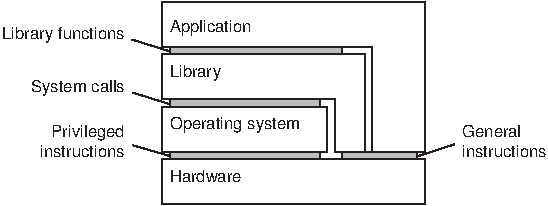
\includegraphics[scale=1.2]{03-06}
  \end{figure}

\end{frame}

\begin{frame}
  \frametitle{Processos VMs vs. Monitores de VM}
  \begin{figure}
    \centering
    \includegraphics[scale=0.83]{03-07}
  \end{figure}

  \begin{itemize}
  \item \textbf{Processos VMs}: um programa é compilado para um código intermediário (portátil) que é executado por um interpretador. Ex: Java VM.
  \item  \textbf{Monitor de VM}: uma camada de software que imita o conjunto de instruções do hardware --- pode executar um sistema operacional completo e suas aplicações. Ex: VMware, VirtualBox.
  \end{itemize}

\end{frame}

\begin{frame}
  \frametitle{Monitores de VM em sistemas operacionais}

  Monitores de VM são executadas em cima de sistemas operacionais existentes.

  \begin{itemize}
  \item Realizam \alert{tradução binária}: enquanto executam uma aplicação ou sistema operacional, traduzem as instruções para as instruções da máquina física
  \item Distinguem \alert{instruções sensíveis}: traps para o núcleo original (system calls ou instruções privilegiadas)
  \item Instruções sensíveis são substituídas por chamadas ao Monitor de VM
  \end{itemize}
\end{frame}



\section{Arquiteturas e Processos de Sistemas Distribuídos}


\setintersectionbg
\begin{frame}[standout]
  \huge{Clientes}
\end{frame}
\setsectionbg


\begin{frame}
  \frametitle{Clientes: interfaces de usuários}
  A maior parte dos softwares do lado do cliente é especializada em interfaces (gráficas) de usuário. O \textit{X protocol} é um exemplo de \textit{thin-client network computing}.

  \begin{figure}
    \includegraphics[width=0.7\textwidth]{03-09}
  \end{figure}
\end{frame}

\begin{frame}
  \frametitle{Software cliente}
  \begin{block}{Geralmente adaptado para transparência de distribuição}
    \begin{itemize}
    \item \alert{transparência de acesso}: \textit{stubs} do cliente para RPC
    \item \alert{transparência de localização/migração}: deixe o software cliente manter o controle sobre a localização atual
    \item \alert{transparência de replicação}: múltiplas evocações são gerenciadas pelo stub do cliente:
      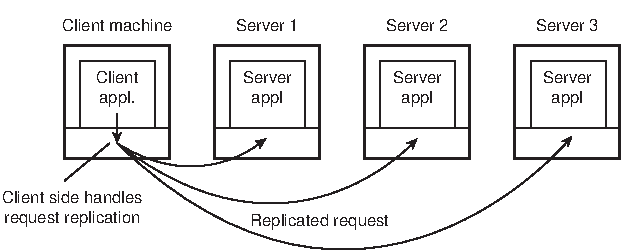
\includegraphics[scale=0.71]{03-10}
    \item \alert{transparência de falhas}: podem geralmente ser responsabilidade só do cliente (que tenta esconder falhas de comunicação e do servidor)
    \end{itemize}
  \end{block}
\end{frame}

\setintersectionbg
\begin{frame}[standout]
  \huge{Servidores}
\end{frame}
\setsectionbg

\begin{frame}
  \frametitle{Servidores: organização geral}

  \begin{block}{Modelo básico}
    Um processo que implementa um serviço específico em nome de uma
    coleção de clientes. Ele espera pela requisição de um cliente,
    garante que a requisição será tratada e, em seguida, passa a
    esperar pela próxima requisição.
  \end{block}
\end{frame}

\begin{frame}
  \frametitle{Servidores concorrentes}
  \begin{block}{Dois tipos básicos:}
    \begin{description}
    \item[Servidores iterativos] o servidor trata uma requisição antes de atender a próxima
    \item[Servidores concorrentes] usa um despachante (\textit{dispatcher}), que pega uma requisição e repassa seu tratamento a uma \textit{thread}/processo separado
    \end{description}
  \end{block}

  \begin{exampleblock}{Observação}
    É mais comum encontrarmos servidores concorrentes: eles podem tratar múltiplas requisições mais facilmente, principalmente se for necessário realizar operações bloqueantes (em discos ou outros servidores).
  \end{exampleblock}
\end{frame}

\begin{frame}
  \frametitle{Servidores: organização geral}

  {\small
    \begin{center}
      \renewcommand{\arraystretch}{1.2}
      \begin{tabular}{|lrl|}\hline
        ftp-data    &     20 &    File Transfer [Default Data]				\\
        ftp         &     21 &    File Transfer [Control]					\\
        telnet      &     23 &    Telnet									\\
        smtp        &     25 &    Simple Mail Transfer						\\
        login       &     49 &    Login Host Protocol						\\
        sunrpc      &    111 &    SUN RPC (portmapper)						\\   \hline
      \end{tabular}
    \end{center}}

  \begin{block}{}
    Cada requisição a uma porta é atribuída a um processo dinamicamente,
    via \emph{superservers} (processo que inicia subprocesso para tratar
    a requisição; ex: UNIX inetd) ou \emph{daemons} (processos que se
    registram em uma porta).
  \end{block}

\end{frame}

\begin{frame}
  \frametitle{Comunicações de controle}
  \begin{block}{Problema:}
    É possível \alert{interromper} um servidor uma vez que ele já tiver aceito (ou estiver processando) uma requisição de serviço?
  \end{block}

  \small
  \begin{block}{Solução 1: usar uma porta diferente para dados urgentes}

    \begin{itemize}
    \item O servidor mantém uma thread/processo separado para mensagens urgentes
    \item Se uma mensagem urgente chegar, a requisição associada é colocada em espera
    \item É necessário que o SO ofereça escalonamento por prioridade
    \end{itemize}
  \end{block}

  \pause

  \begin{block}{Solução 2: usar comunicação de controle da camada de transporte}
    \begin{itemize}
    \item TCP permite o envio de mensagens urgentes na mesma conexão
    \item Mensagens urgentes podem ser recebidas usando tratamento de sinais do SO
    \end{itemize}
  \end{block}

\end{frame}

\begin{frame}
  \frametitle{Servidores e estado}
  \begin{block}{Servidores \textit{stateless}}
    Não mantém informação exata sobre o status de um cliente após ter processado uma requisição:
    \begin{itemize}
    \item Não guarda se um arquivo foi aberto (simplesmente fecha-o e abre de novo se necessário)
    \item Não promete invalidar o cache do cliente
    \item Não rastreia os seus clientes
    \end{itemize}
  \end{block}

  \pause

  \begin{block}{Consequências}
    \begin{itemize}
    \item Clientes e servidores são completamente independentes
    \item \alert{Inconsistências de estado} devido a problemas no cliente ou servidor são reduzidas
    \item Possível \alert{perda de desempenho}. Um servidor não pode antecipar o comportamento do cliente (ex: \textit{prefetching})
    \end{itemize}
  \end{block}

\end{frame}

\begin{frame}
  \frametitle{Servidores e estado}

  \begin{alertblock}{O uso de comunicação orientada a conexão viola o modelo stateless?}
    O uso de conexões com estado não violam o fato de que os
    servidores não guardam estado.

    Mas é necessário ter em mente que a camada de transporte, sim,
    mantém estado. Melhor seria usar um protocolo stateless combinado
    com operações idempotentes\footnote{A idempotência é a propriedade
      que algumas operações têm de poderem ser aplicadas várias vezes
      sem que o valor do resultado se altere após a aplicação
      inicial.}.
  \end{alertblock}

\end{frame}

\begin{frame}
  \frametitle{Servidores e estado}
  \begin{block}{Servidores com estado (\textit{stateful})}

    Guardam o status de seus clientes:
    \begin{itemize}
    \item Registram quando um arquivo foi aberto para realização de \textit{prefetching}
    \item Sabem quando o cliente possui cache dos dados e permitem que os clientes mantenham cópias locais de dados compartilhados
    \end{itemize}
  \end{block}

  \pause
  \begin{alertblock}{Observação:}
    \alert{O desempenho de servidores \textit{stateful} pode ser extremamente alto}, desde que seja permitido que os clientes mantenham cópias locais dos dados. Nesses casos, \alert{confiabilidade não é o maior problema}.
  \end{alertblock}

\end{frame}

\begin{frame}
  \frametitle{Aglomerados de servidores: três camadas diferentes}
  \includegraphics[scale=0.83]{03-12}

  \begin{block}{Elemento crucial}
    A primeira camada é responsável por repassar as requisições para um servidor apropriado.
  \end{block}
\end{frame}

\begin{frame}
  \frametitle{Tratamento de requisições}
  \begin{block}{Observação:}
    Ter uma única camada tratando toda a comunicação de/para o aglomerado pode levar a criação de um \alert{gargalo}.
  \end{block}

  \begin{exampleblock}{Solução:}
    Várias, mas uma popular é o chamado \alert{TCP-handoff}:
  \end{exampleblock}

  \begin{figure}
    \centering
    \includegraphics[scale=0.83]{03-13}
  \end{figure}

\end{frame}

\begin{frame}
  \frametitle{Servidores distribuídos com endereços IPv6 estáveis}
  \begin{figure}[centering]
    \centering
    \includegraphics[scale=0.83]{03-14}\footnote{MIPv6 = Mobile IPV6; HA = Home Address; CA = Care-of Address}
  \end{figure}
\end{frame}

\begin{frame}
  \frametitle{Servidores distribuídos: endereçamento}
  Clientes com Mobile IPv6 podem criar conexões com qualquer outro par de forma transparente:
  \begin{itemize}
  \item Cliente $C$ configura uma conexão IPv6 para o \alert{home address} $HA$.
  \item $HA$ é mantido (no nível da rede) por um \alert{home agent}, que repassa a conexão para um endereço \alert{care-of} $CA$ registrado
  \item $C$ aplica uma \alert{otimização de rota} ao encaminhar os pacotes diretamente para o endereço do $CA$, sem passar pelo \textit{home agent}.
  \end{itemize}

  \pause
  \begin{exampleblock}{CDNs colaborativas}
    O servidor original mantém um \textit{home address}, mas repassa as conexões para o endereço para um servidor colaborador. O original e o colaborador ``parecem'' um único servidor.
  \end{exampleblock}

\end{frame}

\begin{frame}
  \frametitle{Exemplo: PlanetLab}

  \begin{block}{}
    Diferentes organizações contribuem com máquinas, que serão
    \alert{compartilhadas} em vários experimentos.
  \end{block}

  \begin{alertblock}{Problema:}
    É preciso garantir que as diferentes aplicações distribuídas não atrapalhem umas às outras. Solução: \alert{virtualização}.
  \end{alertblock}

\end{frame}

\begin{frame}
  \frametitle{Exemplo: PlanetLab}

  \begin{figure}
    \centering
    \includegraphics{03-15}
  \end{figure}

  \begin{block}{}
    \alert{Vserver:} ambiente independente e protegido com suas
    próprias bibliotecas, versões do servidor, etc. Aplicações
    distribuídas são atribuídas a uma \textbf{coleção} de Vservers
    \alert{distribuídas entre múltiplas máquinas físicas}
    (\textit{slice}).
  \end{block}

\end{frame}

\section{Migração de código}

\begin{frame}
  \frametitle{Migração de código}
  \begin{itemize}
  \item Abordagens para realização de migração de código
  \item Migração e recursos locais
  \item Migração em sistemas heterogêneos
  \end{itemize}
\end{frame}

\newcommand{\STACK}[3]{%
  \framebox[1.6cm]{%
    \begin{minipage}{1.55cm}
      \begin{center}
        \framebox[1.5cm]{\rule{0pt}{0.6em}{#1}} \\
        \framebox[1.5cm]{\rule{0pt}{0.6em}{#2}} \\
        \framebox[1.5cm]{\rule{0pt}{0.6em}{#3}} \\
      \end{center}
    \end{minipage}}}

\begin{frame}{Migração de código: contexto}

  \begin{center}\tiny
    \begin{tabular}{>{\bfseries}lc@{\ }c@{\ }c@{\hspace{3em}}c@{\ }c@{\ }c}
      & \multicolumn{3}{c}{\textbf{Before execution}}
      & \multicolumn{3}{c}{\textbf{After execution}} \\
      & \alert{Client}					& & \alert{Server}
                                        & \alert{Client}					& & \alert{Server} \\ \\
      CS  & \STACK{}{}{}                                        & & \STACK{code}{\alert{state}}{resource}
                                        & \STACK{}{}{}                                        & & \STACK{code}{\alert{state*}}{resource} \\
      \\
      REV & \STACK{code}{}{}				& $\rightarrow$ & \STACK{}{\alert{state}}{resource}
                                        & \STACK{}{}{}					& $\rightarrow$ & \STACK{code}{\alert{state*}}{resource} \\
      \\
      CoD & \STACK{}{\alert{state}}{resource}		& $\leftarrow$ & \STACK{code}{}{}
                                        & \STACK{code}{\alert{state*}}{resource}& $\leftarrow$ & \STACK{}{}{} \\
      \\
      MA        & \STACK{code}{\alert{state}}{resource}	& $\rightarrow$ & \STACK{}{}{resource}
                                        & \STACK{}{}{resource}			& $\rightarrow$ & \STACK{code}{\alert{state*}}{resource} \\
      \\
      \multicolumn{3}{l}{\tiny CS: Cliente--Servidor} &
                                                        \multicolumn{3}{l}{\tiny REV: Remote evaluation} \\
      \multicolumn{3}{l}{\tiny CoD: Code-on-demand} &
                                                      \multicolumn{3}{l}{\tiny MA: Agentes móveis} \\
    \end{tabular}
  \end{center}

\end{frame}

\begin{frame}
  \frametitle{Mobilidade forte e mobilidade fraca}
  \begin{block}{Componentes do objeto:}
    \begin{description}
    \item[Segmento de código] contém o código real
    \item[Segmento de dados] contém o estado
    \item[Estado da execução] contém o contexto das threads executando o código do objeto
    \end{description}
  \end{block}
\end{frame}

\begin{frame}
  \frametitle{Mobilidade forte e mobilidade fraca}
  \begin{block}{Mobilidade fraca}
    Apenas os segmentos de código e dados são migrados (e a execução é reiniciada):
    \begin{itemize}
    \item Relativamente simples, especialmente se o código é portátil
    \item Duas modalidades: \alert{envio de código} (\textit{push}) e \alert{busca de código} (\textit{pull})
    \end{itemize}
  \end{block}

  \begin{block}{Mobilidade forte}
    Move o componente inteiro, incluindo o seu estado de execução.
    \begin{itemize}
    \item \alert{Migração:} move o objeto inteiro de uma máquina para outra
    \item \alert{Clonagem:} inicia um clone e o configura para o mesmo estado de execução.
    \end{itemize}
  \end{block}
\end{frame}

\begin{frame}
  \frametitle{Gerenciamento de recursos locais}
  \begin{alertblock}{Problema:}
    Um objeto usa recursos locais que podem não estar disponíveis no novo local.
  \end{alertblock}

  \begin{block}{Tipos de recursos}
    \begin{description}
    \item[Fixos:] o recurso não pode ser migrado (ex: hardware)
    \item[Anexado:] a princípio o recurso pode ser migrado, mas migração terá alto custo (ex: banco de dados local)
    \item[Desanexado:] o recurso pode ser facilmente movido junto com o objeto (ex: um cache)
    \end{description}
  \end{block}
\end{frame}

\begin{frame}
  \frametitle{Gerenciamento de recursos locais}
  \begin{block}{Ligação objeto--recurso}
    \begin{description}
    \item[Por identificador:] o objeto requer uma instância específica de um recurso (ex: um banco de dados específico)
    \item[Por valor:] o objeto requer o valor de um recurso (ex: o conjunto de entradas no cache)
    \item[Por tipo:] o objeto requer que um determinado tipo de recurso esteja disponível (ex: um monitor colorido)
    \end{description}
  \end{block}
\end{frame}

\begin{frame}{Gerenciamento de recursos locais}

  {\small
    \begin{center}
      \renewcommand{\arraystretch}{1.2}
      \begin{tabular}{|>{\color{red}\bfseries}l|ccc|}\hline
        &	\alert{Desanexado}	&	\multicolumn{1}{c}{\alert{Anexado}}	&	\alert{Fixo}	\\ \hline
        ID		&	MV (ou GR)		&	GR (ou MV)		&	GR                      \\
        Valor	&	CP (ou MV,GR)	&	GR (ou CP)		&	GR                      \\
        Tipo	&	RB (ou MV, GR)	&	RB (ou GR, CP)	&	RB (ou GR)      \\\hline\hline
        \multicolumn{4}{|l|}{\itshape\footnotesize GR = Estabelecer referência global no sistema} \\
        \multicolumn{4}{|l|}{\itshape\footnotesize MV = Mover o recurso} \\
        \multicolumn{4}{|l|}{\itshape\footnotesize CP = Copiar o valor do recurso} \\
        \multicolumn{4}{|l|}{\itshape\footnotesize RB = Religa a um recurso local disponível} \\ \hline

      \end{tabular}
    \end{center}
  }

\end{frame}

\begin{frame}
  \frametitle{Migração em sistemas heterogêneos}
  \begin{block}{Problema principal}
    \begin{itemize}
    \item A máquina destino pode não ser adequada para executar o código migrado
    \item A definição de contexto de thread/processo/processador é \alert{altamente dependente do hardware, sistema operacional e bibliotecas locais}
    \end{itemize}
  \end{block}

  \begin{alertblock}{Única solução}
    Usar alguma \alert{máquina abstrata} que é implementada nas diferentes plataformas:
    \begin{itemize}
    \item Linguagens interpretadas, que possuem suas próximas MVs
    \item Uma MV Virtual (como vimos no início da aula)
    \end{itemize}
  \end{alertblock}

\end{frame}

\begin{frame}
  \frametitle{Migração de uma Máquina Virtual}
  \begin{block}{Migração de imagens: três alternativas}
    \begin{enumerate}
    \item Enviar as páginas de memória para a nova máquina e reenviar aquelas que forem modificadas durante o processo de migração
    \item Interromper a máquina virtual, migrar a memória, e iniciar a nova máquina virtual
    \item Fazer com que a nova máquina virtual recupere as páginas de memória conforme for necessário: processos são iniciados na nova máquina imediatamente e copiam as páginas de memória sob demanda
    \end{enumerate}
  \end{block}
\end{frame}

\begin{frame}
  \frametitle{Desempenho da migração de máquinas virtuais}
  \begin{block}{Problema}
    Uma migração completa pode levar dezenas de segundos. Além disso, é preciso ficar atento ao fato de que um serviço poderá ficar indisponível por vários segundos durante a migração.
  \end{block}

  \begin{figure}
    \centering
    \includegraphics[width=.7\textwidth]{03-26}
    \caption{Medições do tempo de resposta de uma VM durante uma migração}
  \end{figure}
\end{frame}




\end{document}
